\documentclass[12pt]{article}


% Overall formatting
\sloppy
\let\cleardoublepage\clearpage % do not force chapters to start on odd pages


% Graphics
\usepackage{graphicx}
\DeclareGraphicsExtensions{.png,.pdf,.jpg}
\graphicspath{{Figures/}}


\usepackage[a4paper, total={16cm,25cm}]{geometry}



% Tables
\newlength{\mytabskip}   
\setlength{\mytabskip}{-1.5ex}
\newcommand{\tabrule}{\rule[\mytabskip]{0ex}{0ex}}
\usepackage{tabularx}
%\usepackage{longtable}


% bibliography stuff 
\usepackage{natbib}
\bibliographystyle{kluwer} 


\newcommand{\unit}[1]{\ensuremath{\mathrm{#1}}}
\newcommand{\degree}{\ensuremath{\mathrm{^\circ}}}

%\newcommand{\FIXME}[1]{{\sffamily \bfseries #1}}
\newcommand{\FIXME}[1]{{\sffamily {\bfseries \textcolor{red}{FIXME:} #1}}}


\hyphenation{EUMETSAT}
\hyphenation{Metop}



\begin{document}


\thispagestyle{empty}
\noindent
\textbf{\Large Study to support the definition of Arctic Weather \vspace{1mm}\\
Satellite (AWS) high frequency channels} \vspace{8mm}\\
{\bf Patrick Eriksson, Simon Pfreundschuh and Inderpreet Kaur}\\
Department of Space, Earth and Environment\\
Chalmers University of Technology\\
SE-412\,96, Gothenburg, Sweden \vspace{10mm}

\section*{Summary}
%
To written \dots



\setcounter{tocdepth}{1} 
\tableofcontents


\newpage
\setcounter{page}{1}

\section{Introduction}
%
\dots


\section{Assumptions on AWS characteristics}
%
The assumption listed below are primarily taken for the Statement of Work
(SoW), complemented with information provided by Anders Emrich at Omnisys
(private communication, April 14 2020). The later data represent what Omnisys
considers to be technically feasible inside the budget of the project.

\subsection{Channel specifications}
%
Channels around 89, 166, 183 and 229\,GHz are assumed to be fixed, with name,
position and widths defined in Table~\ref{tab:fixed:chs}. AWS channels 31 to 36
will be implemented as a single front-end, but are here still considered as two
``bands'', denoted as 166 and 183\,GHz.

For 325\,GHz, it will be assumed that channels can be placed between 0.75 and
8.0\,GHz in terms of intermediate frequency (IF), and that up to 4 channels
inside this range can be implemented. There should be some gap between these
channels, above 100\,-\,200\,MHz, to facilitate the technical implementation.
For comparison, Table~\ref{tab:fixed:chs} includes also the position of the ICI
325\,GHz channels. As the ICI channels extend to 11\,GHz in IF, they will not
be considered for AWS but will be applied for demonstration and reference
purposes.

For simplicity, the frequency variation of all channel responses is assumed to
be rectangular. This selection shall not be interpreted as any opinion on the
optimal shape of these responses; a significant deviation from a rectangular
shape should be of no concern as long as the actual shape is well
characterised.

\begin{table}[!b]
  \begin{minipage}[b]{0.5\linewidth}
  \centering  
  \begin{tabular}[c]{c|c|c}
    Channel & Frequency   & Bandwidth \\
    name    & [GHz] &  [MHz] \\
    \hline
    AWS-21  & \phantom{0}89.000 & 4000\\
    AWS-31  & 165.500 & 2800\\
    AWS-32  & 176.311 & 2000\\
    AWS-33  & 178.811 & 2000\\
    AWS-34  & 180.311 & 1000\\
    AWS-35  & 181.511 & 1000\\
    AWS-36  & 182.311 & \phantom{0}500\\
    AWS-41  & 229.000 & 2000\\
    \hline
  \end{tabular}
  \end{minipage}%
  \begin{minipage}[b]{0.5\linewidth}
  \centering  
  \begin{tabular}[c]{c|c|c}
    Channel & Frequency   & Bandwidth \\
    name    & [GHz] &  [MHz] \\
    \hline
    ICI-5  & 325.15$\pm$9.50 & 3000\\
    ICI-6  & 325.15$\pm$3.50 & 2400\\
    ICI-7  & 325.15$\pm$1.50 & 1600\\
    \hline
  \end{tabular}
  \end{minipage}  
  \caption{Fixed channel position and widths. The left table covers channels of
    AWS, with values taken from SoW. Channels AWS-21 to AWS-36 are at this
    moment mandatory for AWS, while AWS-41 is so far tentative. The right table
    lists the values of some channels of ICI \citep{eriksson:towar:20}.}
  \label{tab:fixed:chs}
\end{table}


\subsection{Noise}
%
The nominal reciever noise temperature, $T_r$ of each band is listed in
Table~\ref{tab:trec}. The noise of data for individual channels is calculated
as
\begin{equation}
  \sigma^i = c \frac{T^i_r+T^i_a}{\sqrt{\Delta\!f^i\Delta t}}
\end{equation}
where $\sigma^i$ is the noise standard deviation of channel $i$, $c$ is a
scaling factor (see below), $T^i_r$ is the reciever noise temperature of the
channel, $T^i_a$ is the antenna temperature of the channel, $\Delta\!f^i$ is the
bandwidth of channel and $\Delta t$ is the integration time.

The factor $c$ is set to 1.2 to incorporate the additional noise caused by the
calibration process. The bandwith applied is the one found in columns 3 of
Table~\ref{tab:fixed:chs}. The integration time is set to match an effective
15\,km resolution at 183\,GHz. This time was estimated to 3\,ms. 

\begin{table}[!bt]
  \centering
  \begin{tabular}[b]{c|ccccc}
    Band [GHz]   & 89 & 166 & 183 & 229 & 325 \\
    \hline
    $T_r$ [K]    & 390 & 650 & 650 & {\it 1000}  & 1200 \\
    \hline
  \end{tabular}
  \caption{Assumed reciever noise temperatures. The value for 229\,GHz is
    selected by us, remaining values are present assumptions at Omnisys.}
  \label{tab:trec}
\end{table}

\subsection{Various}
%
The AWS satellite is assumed to be at an altitude of 600\,km. Data were
generated for sensor viewing angles (the angle from nadir) from 0$^\circ$ to
45$^\circ$, in steps of 5$^\circ$.

The polarisation response of the bands is not yet determined and for simplicity
``quasi-horisontal'' (defined in same way as for e.g.\ MWS) is throughout
assumed. Antenna temperatures are obtained as:
\begin{equation}
  \label{eq:polrot}
  T_a = T_b^V\sin^2(\theta) + T_b^H\cos^2(\theta)
\end{equation}
where $T_b^V$/$T_b^H$ is the brightness temprature at vertical/horisontal
polarisation, respectively, and $\theta$ is the viewing angle (from nadir).



\section{Input data and software}

\subsection{Atmospheric scenarios}

\subsubsection{Fascod}
\label{sec:fascod}
%
The Fascod dataset \citep{anderson1986afgl} was used to represent different
climate zones in overview calculations. The dataset consists of profiles of
pressure, temperature and volume mixing ratio profiles of various atmospheric
gases. Five climatoligies were used: tropical (TRO), mid-latitude summer (MLS),
mid-latitude winter (MLW), sub-arctic summer (SAS), and sub-arctic winter
(SAW). No hydrometeors were included in simulations involving Fascod.


\subsubsection{Bulk profile database}
%
A database of atmospheric cases was created based on data from CloudSat and
ERA-Interim. The core idea of the approach is to use CloudSat reflectivities to
obtain as realistic vertical profiles of ice hydrometeors and rain as
possible. No external CloudSat retrievals are involved. Instead the CloudSat
reflectivites are mapped to properties for the passive simulations by assuming
a particle size distribution (PSD) and a particle habit, together denoted as
the particle model. The process involves an inversion of the radar data, but as
the same particle model is used for that inversion and to map ice water content
(IWC) and rain water content (RWC) to single scattering data when performing
the passive radiative transfer calculations, the impact of clouds on the
simulated AWS data is as realistic as possible. The thin clouds not detected by
CloudSat should not be of relevance for passive measurements frequencies
350\,GHz. Background data (temperature, humidity, 10\,m wind speed, \dots) were
taken from ERA-Interim, for the time and location of the CloudSat data. Liquid
water content (LWC) was taken from ERA-Interim, as CloudSat has no sensitivity
to the hydrometeor category.

This approach for generating atmospheric scenarios has been used by us since
\citet{rydberg:nonga:09}, and more recently in e.g.\
\citet{eriksson:towar:20,barlakas:three:20}. It is also used in
\citet{ekelund:using:20}, where the approach is described more in detail. In
the cited articles, the sensor's footprint has been considered in varying
degree, as ``beam filling'' must be considered at high impact of hydrometeors.
As clear-sky and weak cloud interference are in focus in this study, and to
save calculation time, instead CloudSat data were averaged over 10\,km to form
the atmospheric cases and standard 1D radiative transfer calculations are
applied on each case (instead of applying an independent beam approximation
inside a 2D or 3D atmosphere as done in cited works).

[* Do we show comparison to ATMS, or do we refer to articles for ``validation''? ]
[* Add time and latitude ranges used * ]


\subsection{Radiative transfer simulations}
%
\subsubsection{ARTS}
%
All radiative transfer calculations are made by the Atmospheric Radiative
Transfer System (ARTS, \citet{eriksson:arts2:11,buehler:artst:18}), version
arts-2.3.????. Models and input used for absorption and hydrometeor properties
are described below. Ocean/water and land emissivities are taken from
TESSEM \citet{prigent2017sea} and TELSEM \citet{aires2011tool}, respectively.

The calculations were performed for each atmospheric cases. One ''clear-sky''
where all hydrometeors contents were set to zero, and one ``all-sky'' where IWC
and RWC derived from CloudSat reflectivities and LWC from ERA-Interim were
included. Both sets of calculations were were made by ARTS's interface to the
RT4 solver \citep{evans1995microwavec}. This ``scattering solver'' was used
also for clear-sky, to avoid a possible bias between clear-sky and all-sky for
insignificant hydrometeor contents. RT4 handles the first two elements of the
Stokes vector, that were converted to brightness temperatures for H- and V-
polarisation.


\subsubsection{Absorption models}
%
The absorption of nitrogen is modelled following \citet{pwr:93}. Nitrogen has a
significant impact at least around 325\,GHz at dry conditions. Also oxygen
absorption follows \citet{pwr:93}. Oxygen is in this study mainly of concern
for the 89\,GHz CloudSat simulations. LWC was treated to be
purely absorbing, based on \citet{ellison2007permittivity}.

For water vapour the present settings in RTTOV are applied. That is, largely
MPM89 \citep{liebe:89} is followed, but some parameters for the 22 and 183\,GHz
transitions are replaced \citep{saunders2018update,turner2019amsutran}. A basic
comparison to RTTOV (12.?) was made (with MHS as assumed sensor) and an
agreement around or better than 0.?\,K was found.


\subsubsection{Hydrometeor properties}
%
[* Write later, Simon? TRO only! *]


\section{Overview of the 183, 229 and 325\,GHz bands}
%
The simulations in this section are based on five Fascod climate scenarios
(Sec.~\ref{sec:fascod}), and performed with a fixed sensor viewing angle of
25$^\circ$. No hydrometeors are included. For simpler interpretation of the
results, the reflectivity is set to have no frequency variation, i.e.\ the same
value is applied for all bands. The reflective is varied between 0 and 0.5.
In the figures covering transmissivities and Jacobians, the specifications
of ICI is applied for 325\,GHz channels (Table~\ref{tab:fixed:chs}).


\subsection{Clear-sky brightness temperatures}
%
Figure~\ref{fig:tb:r000} shows brightness temperatures over the three bands, for
a reflectivity of 0 (i.e.\ a blackbody surface). The figure takes into account
that the 183\,GHz channels of AWS are of single-sideband character, while for
229 and 325\,GHz averages of upper and lower sidebands are shown, plotted as
a function from the centre frequency on the lower side.

\begin{figure}[p]
  \centering
  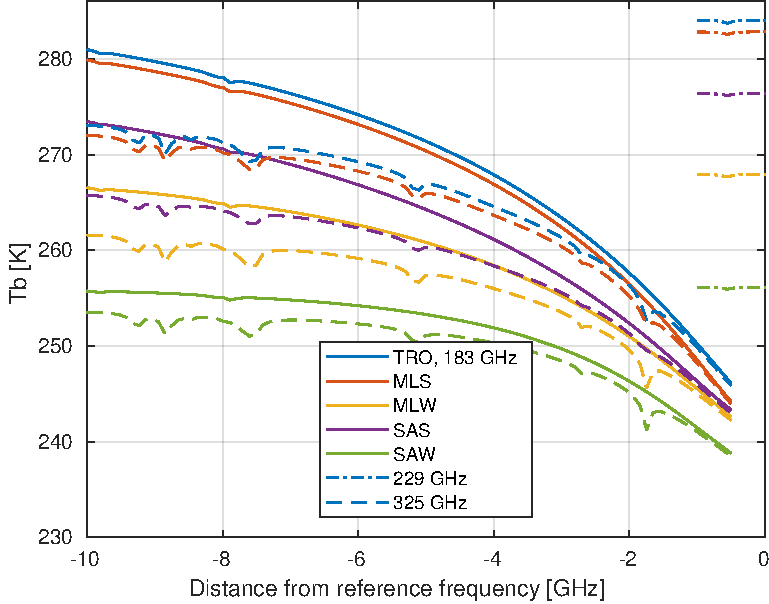
\includegraphics[width=0.75\textwidth]{fascod_tb_r000}
  \caption{Solid lines show brightness temperatures for the lower wing of the
    183.31\,GHz transition. Dashed lines represent double-sideband measurements
    around 325.15\,GHz, with the mean of upper and lower band shown on the low
    side. Dash-dotted lines represent double-sideband measurements around
    229.00\,GHz in the same manner, but only over the bandwidth of the
    potential channel. For all three bands, spectra for all five
    Fascod scenarios are included.}
  \label{fig:tb:r000}
\end{figure}
\begin{figure}[p]
  \centering
  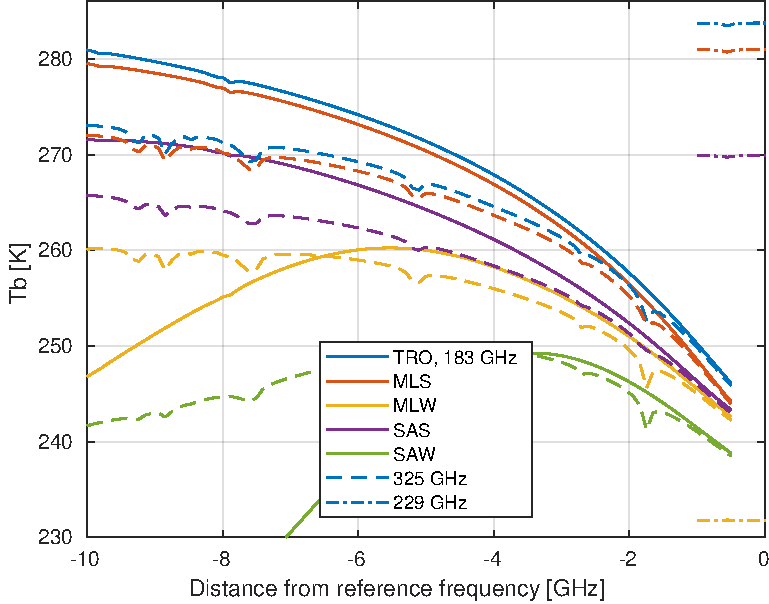
\includegraphics[width=0.75\textwidth]{fascod_tb_r050}
  \caption{Same as figure above, but with a surface reflectivity of 0.5.}
  \label{fig:tb:r050}
\end{figure}
\begin{figure}[p]
  \centering
  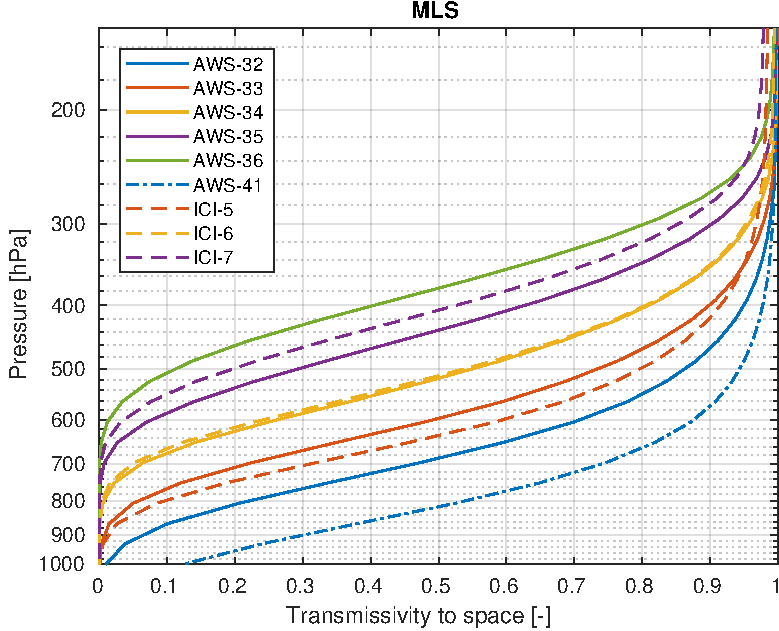
\includegraphics[width=0.75\textwidth]{fascod_tr_mls}
  \caption{Transmissivity to space as a function of altitude, for the
    mid-latitude summer scenario. Solid lines represent 183\,GHz channels,
    dashed lines 325\,GHz channels and dashed-dotted the 229\,GHz channel
    (Table~\ref{tab:fixed:chs}). These transmissivities are independent of
    surface reflectivity.}
  \label{fig:tr:mls}
\end{figure}
\begin{figure}[p]
  \centering
  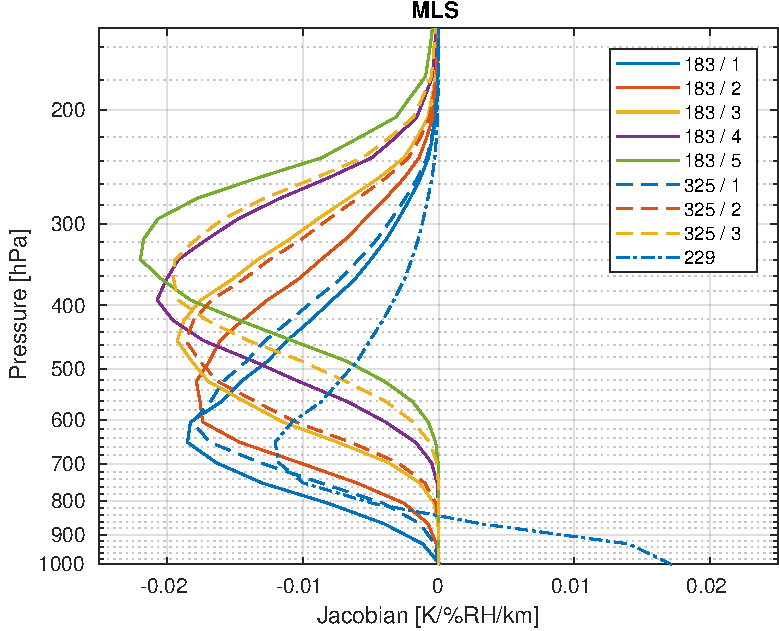
\includegraphics[width=0.75\textwidth]{fascod_wf_mls_025}
  \caption{Jacobians for relative humidity. Line symbols as in Fig.~\ref{fig:tr:mls}.
    Surface reflectivity is set to 0.25.}
  \label{fig:wf:mls:025}
\end{figure}

For 183 and 325\,GHz the brightness temperatures increase when moving away from
the centre frequency of the transition. The ``kinks'' in the spectra correspond
to ozone transitions, that are both more frequent and stronger in the 325\,GHz
range than in the 183\,GHz one. See Fig.~1 of \citet{eriksson:towar:20} for how
the ozone transitions are distributed between the lower and upper 325\,GHz
sideband. The spectra of 183 and 325\,GHz deviate little close to the transition
frequency, showing that the two frequencies are of similar strength, though the
325\,GHz one is slightly weaker. The higher deviations further out in the wings
are due to different contribution of far wing and continuum absorption, that is
higher at 325\,GHz. The 229\,GHz brightness temperatures is higher than any
value around 183 and 325\,GHz, as expected 229\,GHz being a window channel.

In Figure~\ref{fig:tb:r050} the surface reflectivity is changed to 0.5, which
should roughly correspond to the highest reflectivity encountered at these
frequencies. The differences to Fig.~\ref{fig:tb:r000}  are small for 183 and
325\,GHz for the tropical and the two summer scenarios. On the other hand,
there is a clear impact in the wing part of 183\,GHz for the two winter
scenarios. The same is true for 340\,GHz, but the influence of the surface
reflectivity is considerably lower. [* Comment somewhere on the implications of
this for retrievals at high latitudes *] Beside for the tropical case, for
229\,GHz there is a pronounced dependency of the surface reflectivity, e.g.\
about 35\,K for mid-latitude winter.


\subsection{Clear-sky transmissivities to space}
%
Assuming that a cloud layer can be moved in altitude, its impact on measured
brightness temperatures will roughly follow the transmissivity to space for the
cloud altitude. In short, where the transmissivity is zero the cloud will have
no impact, while where the transmissivity is unity the influence will be close
to constant with altitude (especially when the single scattering albedo is
high). This relationship just refers to the relative impact for a
given frequency, the absolute impact (at transmissivity 1) increases in general
with frequency. 

Figure~\ref{fig:tr:mls} displays examples on transmissivities to space. The
transmissivities refers to the up-welling radiation. The contribution from
reflected down-welling is neglected and the considered transmissivity does not
depend on surface reflectivity.

The altitude variation of transmissivity exhibits same basic shape between all
the 183 and 325\,GHz channels, but the altitude of optical thickness of 1
(transmissivity of $e^{-1}\approx0.37$) varies. The curves of the edge 183\,GHz
channels (AWS-32 and 36) brackets the ones corresponding to the ICI 325\,GHZ
channels. The later channels show a higher deviation from 1 at 150\,hPa, due to
some (weak) ozone attenuation in the stratosphere. The 229\,GHz has the highest
transmissivities.


\subsection{Clear-sky relative humidity weighting functions}
%
The sensitivity to humidity is most easily compared by the channels' weighting
functions (i.e.\ the Jacobian), and examples are found in
Fig.~\ref{fig:wf:mls:025}. The shape of the weighting functions depends on the
unity selected for representing water vapour. As the absolute amount of water
vapour varies with orders of magnitude from the surface to the tropopause, it
is difficult to interpret weighting functions for absolute humidity units and
it is more suitable to use a relative one. In Fig.~\ref{fig:wf:mls:025} the
weighting functions correspond to an increase of relative humidity (RH) with one
percent unit over 1\,km. RH with respect liquid/ice is applied above/below
0$^\circ$C.

The basic shape of the Jacobian is similar for all 183 and 325\,GHz channels,
but the peak altitude varies. Again the edge 183\,GHz channels brackets the
325\,GHz ICI ones, as for transmissivity. These Jacobians are negative, meaning
that a change towards higher humidity results in decreased brightness
temperatures. The 229\,GHz Jacobian is positive close to the surface, as this
channel has sensitivity all the way down to the surface and more water vapour
just above a reflecting surface results in higher brightness temperatures. The
switch from negative to positive Jacobian depends on atmospheric scenario and
surface reflectivity. For dry conditions also the outer 183 and 325\,GHz
channels can have a positive part, as long as the reflectivity is not close to
0.


\section{Preliminary options for 325\,GHz channels}

\subsection{...}
%
\dots Fig.~\ref{fig:wfuns:325ul}

\begin{figure}[!tb]
  \centering
  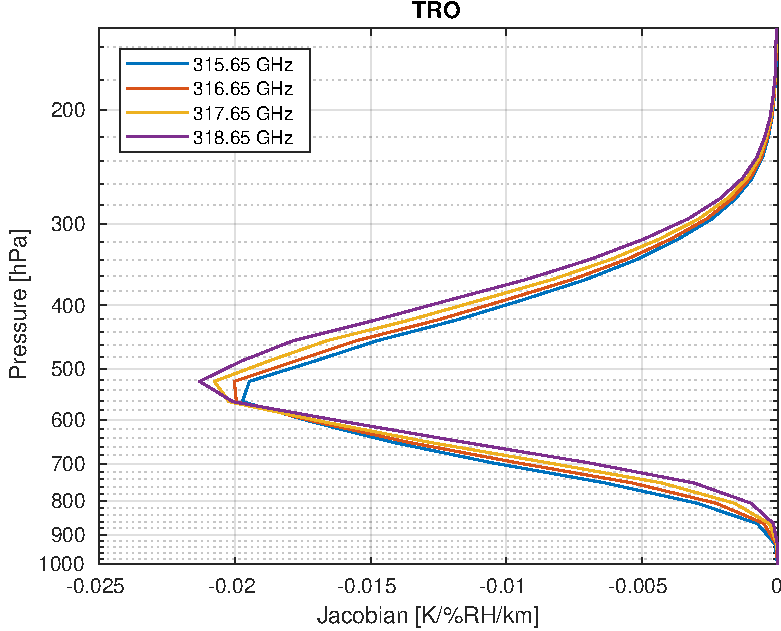
\includegraphics[height=65mm]{fascod_wf_325l_tro}\hspace{5mm}% 
  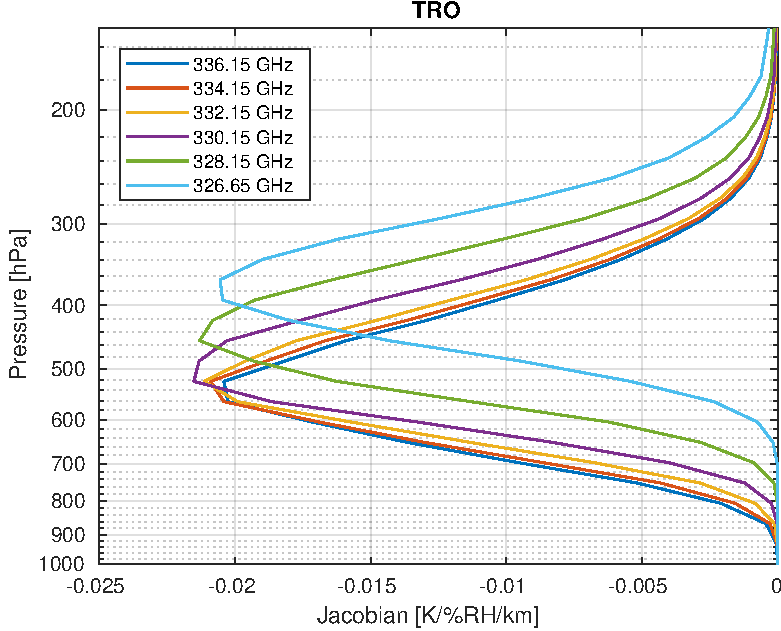
\includegraphics[clip,trim=43 0 0 0,height=65mm]{fascod_wf_325u_tro}
 \caption{...}
  \label{fig:wfuns:325ul}
\end{figure}





\section{Notes}
\begin{itemize}
\item Discuss selection of polarisation
\end{itemize}

{\footnotesize
\bibliography{j_abbr,references}
}

\end{document}
